% Copyright 2004 by Till Tantau <tantau@users.sourceforge.net>.
%
% In principle, this file can be redistributed and/or modified under
% the terms of the GNU Public License, version 2.
%
% However, this file is supposed to be a template to be modified
% for your own needs. For this reason, if you use this file as a
% template and not specifically distribute it as part of a another
% package/program, I grant the extra permission to freely copy and
% modify this file as you see fit and even to delete this copyright
% notice. 

% \UseRawInputEncoding
\documentclass{beamer}

% There are many different themes available for Beamer. A comprehensive
% list with examples is given here:
% http://deic.uab.es/~iblanes/beamer_gallery/index_by_theme.html
% You can uncomment the themes below if you would like to use a different
% one:
%\usetheme{AnnArbor}
%\usetheme{Antibes}
%\usetheme{Bergen}
%\usetheme{Berkeley}
%\usetheme{Berlin}
%\usetheme{Boadilla}
%\usetheme{boxes}
%\usetheme{CambridgeUS}
%\usetheme{Copenhagen}
%\usetheme{Darmstadt}
%\usetheme{default}
%\usetheme{Frankfurt}
%\usetheme{Goettingen}
%\usetheme{Hannover}
%\usetheme{Ilmenau}
%\usetheme{JuanLesPins}
%\usetheme{Luebeck}
\usetheme{Madrid}
%\usetheme{Malmoe}
%\usetheme{Marburg}
%\usetheme{Montpellier}
%\usetheme{PaloAlto}
%\usetheme{Pittsburgh}
%\usetheme{Rochester}
%\usetheme{Singapore}
%\usetheme{Szeged}
%\usetheme{Warsaw}

\usepackage{pgfgantt}
\usepackage{todonotes}
\usepackage{media9}
\usepackage{fontawesome5}
\usepackage{subfigure}
\usepackage{booktabs,array}
\usepackage{tabulary}
\usepackage{caption}
\usepackage{subfigure}
\usepackage{siunitx}

\usepackage[ruled, vlined, linesnumbered]{algorithm2e} % For algorithms

\usepackage{amsmath} % For typesetting math

% Customize Warsaw color 
\setbeamercolor*{palette primary}{use=structure,fg=white,bg=red!50!black}
\setbeamercolor*{palette secondary}{use=structure,fg=white,bg=red!60!black}
\setbeamercolor*{palette tertiary}{use=structure,fg=white,bg=red!70!black}

% Customize Warsaw block title and background colors
\setbeamercolor{block title}{bg=red!50!black,fg=white}

\setbeamertemplate{bibliography item}{\insertbiblabel}  % insert bibliography numbers instead of symbol
\setbeamertemplate{caption}[numbered] % adds the figure or table number to the caption.



\title[Robotic Cart System (Proposal)]{Robotic Cart System}

% % A subtitle is optional and this may be deleted
\subtitle{Product Proposal}

\author[K.~Allen, D.~Beebe, J.~Braker]{Kallistah~Allen \and Darrah~Beebe \and
Jason~Braker
Advisors:~Dr.~Suruz~Miah \and Dr.~Prasad~Shastry}
% - Give the names in the same order as the appear in the paper.
% - Use the \inst{?} command only if the authors have different
%   affiliation.

\institute[Bradley University] % (optional, but mostly needed)
{
  Department of Electrical and Computer Engineering\\
  Bradley University\\
  1501 W. Bradley Avenue\\
  Peoria, IL, 61625, USA
}
% - Use the \inst command only if there are several affiliations.
% - Keep it simple, no one is interested in your street address.

% \date[November~10,~2020]{Tuesday, November~10,~2020}

% - Either use conference name or its abbreviation.
% - Not really informative to the audience, more for people (including
%   yourself) who are reading the slides online

\logo{\hfill\href{http://www.bradley.edu}{
\includegraphics[width=0.75cm]{figs/logoBU1-Print}}}  % place logo in every page 


% \subject{Mobile Robot Localization}
% This is only inserted into the PDF information catalog. Can be left
% out. 

% If you have a file called "university-logo-filename.xxx", where xxx
% is a graphic format that can be processed by latex or pdflatex,
% resp., then you can add a logo as follows:

% \pgfdeclareimage[height=0.5cm]{university-logo}{university-logo-filename}
% \logo{\pgfuseimage{university-logo}}

% Delete this, if you do not want the table of contents to pop up at
% the beginning of each subsection:
\AtBeginSubsection[]
{
  \begin{frame}<beamer>{Outline}
    \tableofcontents[currentsection,currentsubsection]
  \end{frame}
}

% Let's get started
\begin{document}

\begin{frame}
  \titlepage
\end{frame}

\begin{frame}{Outline} 
  \tableofcontents%[pausesections]
  % You might wish to add the option [pausesections]
\end{frame}

% Section and subsections will appear in the presentation overview
% and table of contents.
\section{Introduction}

\begin{frame}{Introduction}
  \begin{center}
    \href{videos/proposalVideo.mp4}{
\includegraphics[width=0.8\textwidth]{figs/img/proposalVideoTitle}}
  \end{center}
  %%% Embedding the video with the includemedia command below would be nice, but I could not get it to work correctly - JB
  % \begin{center}
  %   \includemedia[
  %     width=\textwidth,
  %     height=0.7\textheight,
  %     label=proposalVideo,
  %     % activate=onclick,
  %     % playbutton=fancy,
  %     addresource=videos/proposalVideo.mp4,
  %     flashvars={source=videos/proposalVideo.mp4}]
  %     {}{VPlayer.swf}
  %     \\
  %     % \mediabutton[
  %     %   mediacommand=proposalVideo:playPause,
  %     %   overface=\color{blue}{\fbox{\strut \faPause\ \faPlay}},
  %     %   downface=\color{red}{\fbox{\strut \faPause\ \faPlay}}
  %     % ]{}
  %     % \mediabutton[
  %     %   mediacommand=proposalVideo:setSource
  %     %   [(videos/proposalVideo.mp4)]]{\fbox{Introduction Video}}
  % \end{center}
\end{frame}

\begin{frame}{Introduction}{}
  % applications of mobile robot navigation and problem description
  \begin{block}{Applications of Mobile Carts}
    \begin{itemize}
      \item Mail delivery
      \item Transferring files in offices
      \item Carrying medical supplies in Hospitals
      \item Carrying materials and tools on construction sites
      \item Shopping carts for ease of use and people with disabilities
    \end{itemize}
  \end{block}
\end{frame}

%----------------------------------

\begin{frame}{Introduction}

  \begin{block}{Problem Statement}
  In this project, we are proposing a robotic cart that would primarily utilize analog signals along with cost-effective wireless communication to identify the customer and be able to track and follow the customer through the store.
  \end{block}
\end{frame}

%----------------------------------

\section{Literature Review}

\begin{frame}{Literature Review}
  \begin{block}{Existing Solutions}
    \begin{itemize}
        \item Methods of tracking a customer and following them through the store
            \begin{itemize}
                \item Mobile platform interface with ultrasound and radio transmission technology
                \item Gated Recurrent Unit (GRU) network with LiDAR sensor and camera to map the customer
                \item Arduino MEGA 2560, six ultrasonic sensors, two DC motors with Pulse Width Modulation (PWM), an Android Studio IDE device, and Bluetooth
            \end{itemize}
       % \item Block Diagram shown in Figure \autoref{fig:sysBlockDiag}
    \end{itemize}
  \end{block}
    %\begin{figure}[b]
     %   \centering
     %   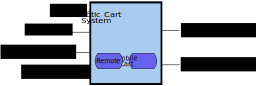
\includegraphics[width=\textwidth]{figs/system_block_diagram}
     %   \caption{Block Diagram of the Robotic Cart System}
     %   \label{fig:sysBlockDiag}
    %\end{figure}
\end{frame}

%----------------------------------

\begin{frame}{Literature Review}
  Existing Solutions:
  
  \begin{figure}
    \centering
    \begin{minipage}[t]{0.32\textwidth}
      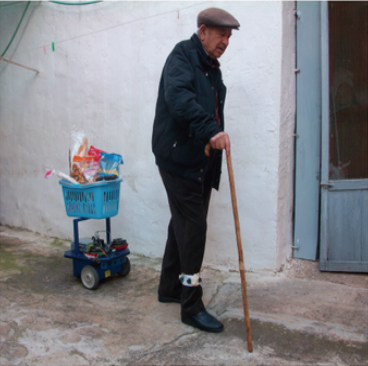
\includegraphics[width=1\textwidth]{figs/img/CompaRob}
      \caption{CompaRob}
      % \label{fig:budgetBotChassis}
    \end{minipage}%
    \begin{minipage}[t]{0.32\textwidth}
      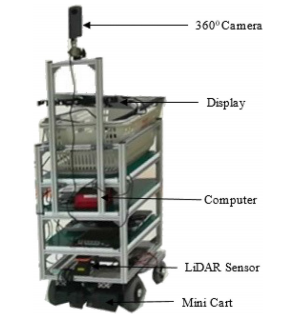
\includegraphics[width=1\textwidth]{figs/img/ShoppingSuportRobot}
      \caption{Shopping Support Robot}
      % \label{fig:beagleboneBlue}
    \end{minipage}
    \begin{minipage}[t]{0.32\textwidth}
      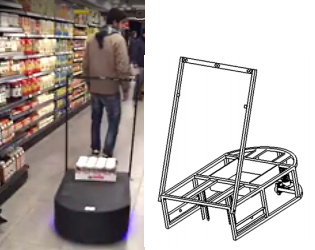
\includegraphics[width=1\textwidth]{figs/img/SmartCart}
      \caption{Smart Cart Robot}
      % \label{fig:XBeeModule}
    \end{minipage}
  \end{figure}
\end{frame}

%----------------------------------

\begin{frame}{Literature Review}
  \begin{block}{Multipath Interference}
    \begin{itemize}
      \item Proposed solutions to multipath interference
      \begin{itemize}
        \item Course estimation calculations such as recieved signal strength indicator (RSSI) and time difference of arrival (TDoA)
        \item IEEE 802.11b wireless Ethernet device to measure RF signals
        \item Sampling radio signal strength (RSS) at discrete points without too much deviation from the robot's desired position
      \end{itemize}
    \end{itemize}
  \end{block}
\end{frame}

%----------------------------------

\begin{frame}{Literature Review}
  \begin{block}{Challenges}
    \begin{itemize}
      \item Communication between the robot and the remote
      \item Buffer distance between the robotic cart and the customer without using line of sight sensing
    \end{itemize}
  \end{block}
\end{frame}

%----------------------------------

\section{Functional Requirements}
\subsection{System Architecture}
\begin{frame}{System Architecture}
  \begin{itemize}
    \item Mobile robot (Budget Bot)
    \item BeagleBone Blue interface
    \item XBee wireless communication from the mobile robot to the remote target
  \end{itemize}
  
  \begin{figure}
    \centering
    \begin{minipage}[t]{0.32\textwidth}
      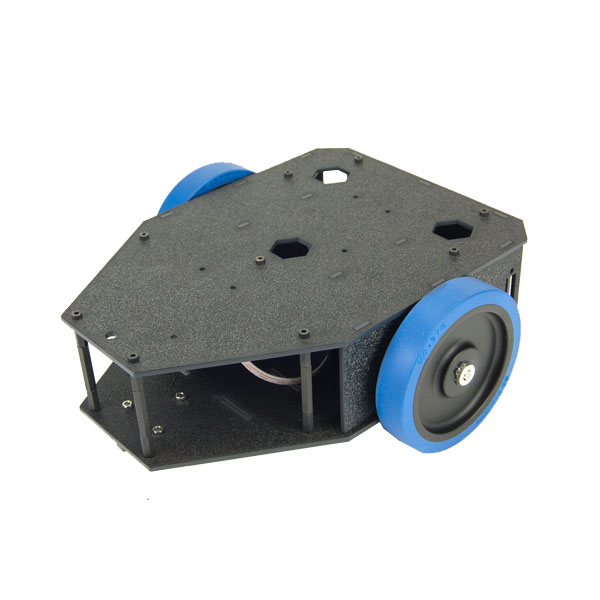
\includegraphics[width=1\textwidth]{figs/img/budgetbot_chassis}
      \caption{Budget Bot Chassis}
      % \label{fig:budgetBotChassis}
    \end{minipage}%
    \begin{minipage}[t]{0.32\textwidth}
      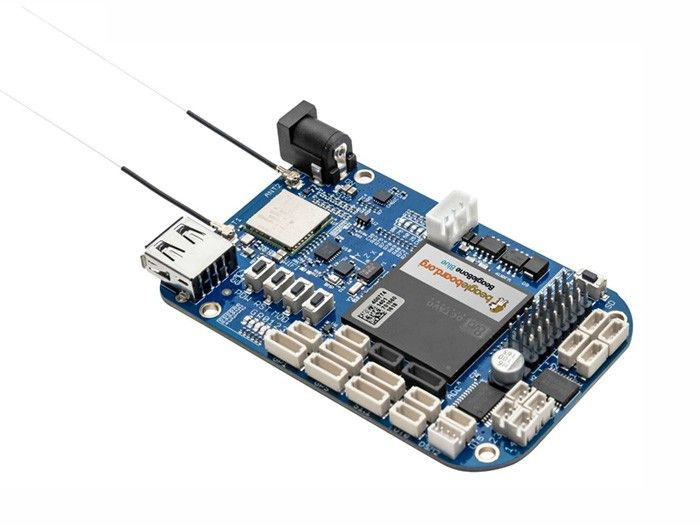
\includegraphics[width=1\textwidth]{figs/img/beaglebone_blue}
      \caption{BeagleBone Blue}
      % \label{fig:beagleboneBlue}
    \end{minipage}
    \begin{minipage}[t]{0.32\textwidth}
      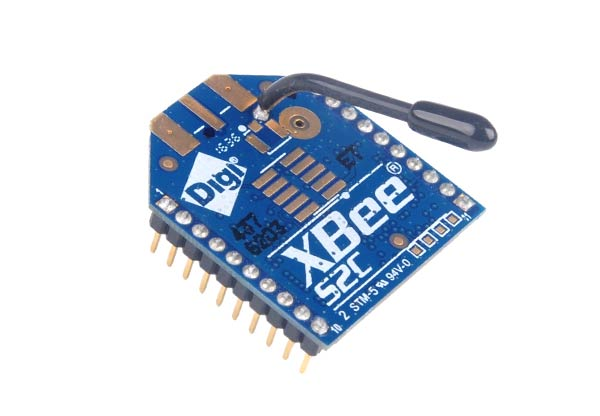
\includegraphics[width=1\textwidth]{figs/img/Xbee-S2C-Module}
      \caption{XBee S2C Module}
      % \label{fig:XBeeModule}
    \end{minipage}
  \end{figure}
\end{frame}

%----------------------------------

\begin{frame}{System Architecture}
  Model of the Budget Bot for CoppeliaSim Simulation:
  \begin{figure}[b]
    \centering
    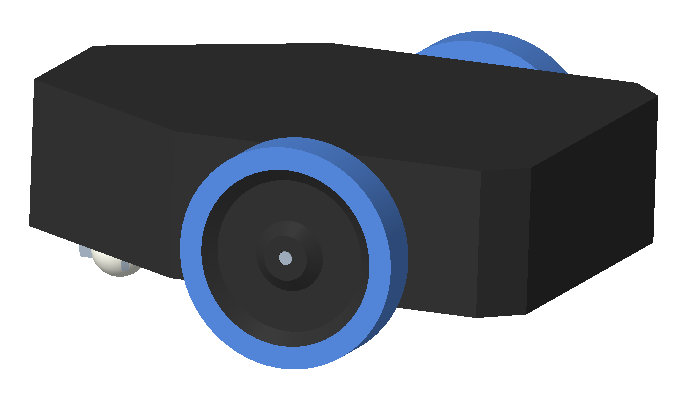
\includegraphics[width=0.75\textwidth]{figs/img/budgetBotModel}
    \caption{Budget Bot Chassis}
    \label{fig:coppeliasimModel}
  \end{figure}
\end{frame}

%----------------------------------

\begin{frame}{System Architecture}
    \begin{block}{Reflector Design}
    Two designs for reflector array:
    \begin{itemize}
      \item Paraboloidal Reflector (Fig. \ref{fig:parabolodialReflector})
      \item Combined Parabolic/Paraboloidal Reflector (Fig. \ref{fig:parabolicReflector})
    \end{itemize}
    \end{block}
    \begin{figure}
      \centering
      \begin{minipage}[t]{0.5\textwidth}
        \centering
        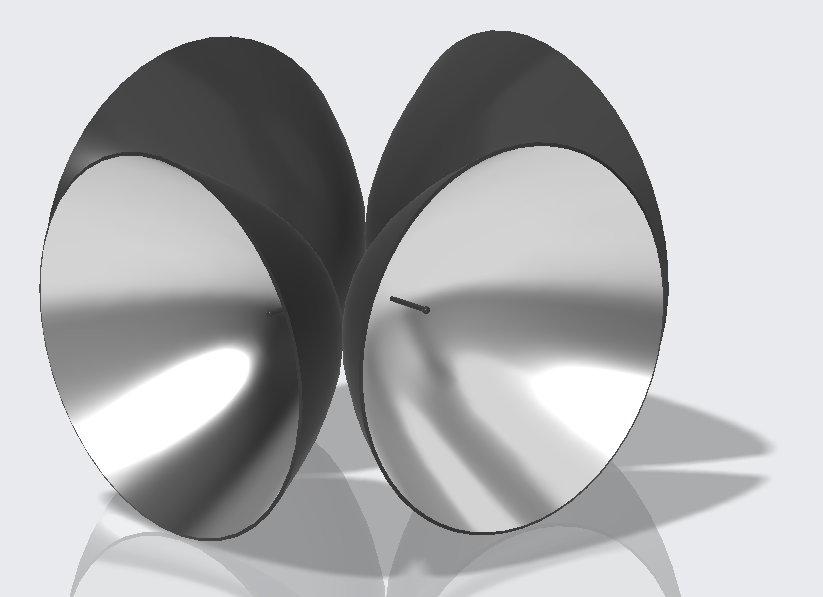
\includegraphics[height=3.5cm]{figs/img/paraboloidalReflector}
        \caption{Paraboloidal Reflector Model}
        \label{fig:parabolodialReflector}
      \end{minipage}
      \begin{minipage}[t]{0.4\textwidth}
        \centering
        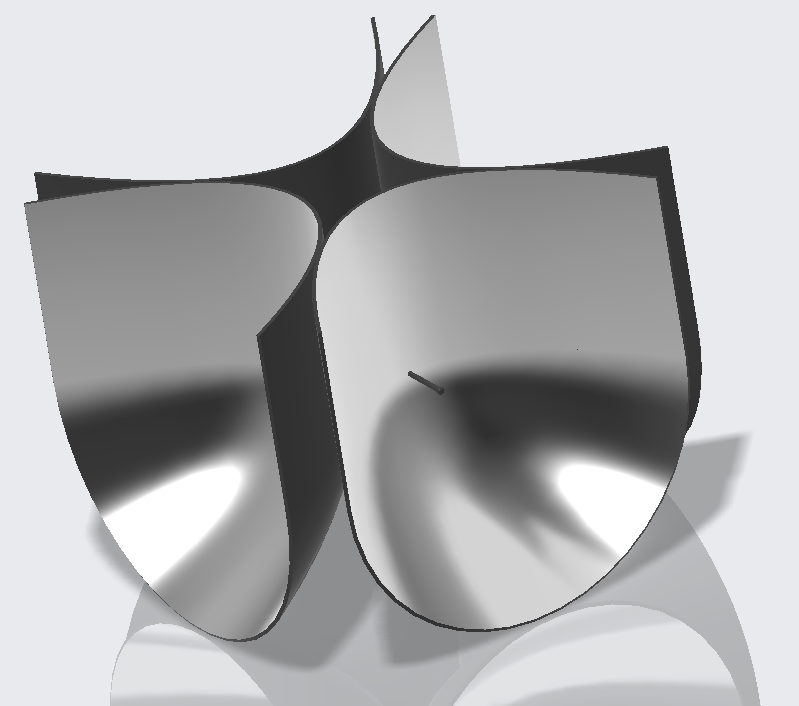
\includegraphics[height=3.5cm]{figs/img/parabolicReflector}
        \caption{Combined Parabolic/Paraboloidal Reflector}
        \label{fig:parabolicReflector}
      \end{minipage}
    \end{figure}
\end{frame}

%----------------------------------

% \begin{frame}{System Architecture}
%     % Navigation Algorithm
%     \begin{algorithm}
%       \SetAlgoLined
%       \KwIn{
%         \begin{itemize}
%           \item Distance $d_{Ref}$ between robot and remote
%           \item Angle $\theta_{Ref}$ of the remote with respect to robot's local coordinate frame
%         \end{itemize}}
%       \KwOut{Mobile Robot Trajectory}
%       \Begin
%       {
%         Initialize robot pose $q_0 = [x_0, y_0, \theta_0]^T$\\
%         Initialize robot parameters, sampling time $T > 0$, $K_p$, $K_\omega$\\
%         Initialize time index $k = 0$\\
%         Set total number of simulation time steps $k_f$\\
%         \While{$k \leq k_f$}
%         {
%           $t = kT$\\
%           Compute coordinates of target point with respect to robot's local frame as $x_{Ref} = (d_{Ref} - 1)\cos \theta_{Ref}$, $y_{Ref} = (d_{Ref} - 1)\sin \theta_{Ref}$\\
%           Compute linear speed $v(t) = sign(xRef)K_p\sqrt{x_{Ref}^2 + y_{Ref}^2}$\\
%           Compute $\omega(t) = K_\omega \theta_{Ref}$\\
%           Compute left and right wheel speeds for robot\\
%           Apply wheel speeds to robot for sampling time $T$\\
%           $k = k + 1$
%         }
%       }
%       \caption{Modified Point Navigation Algorithm}
%       \label{alg:remoteTracking}
%     \end{algorithm}
% \end{frame}

%----------------------------------

\begin{frame}{System Architecture}
    \begin{block}{Proposed Demonstration of the Robotic Cart Project}
    Draft demonstration of how the Robotic Cart project will run once all the components are assembled
    \end{block}
    %\begin{figure}[b]
    %    \centering
    %    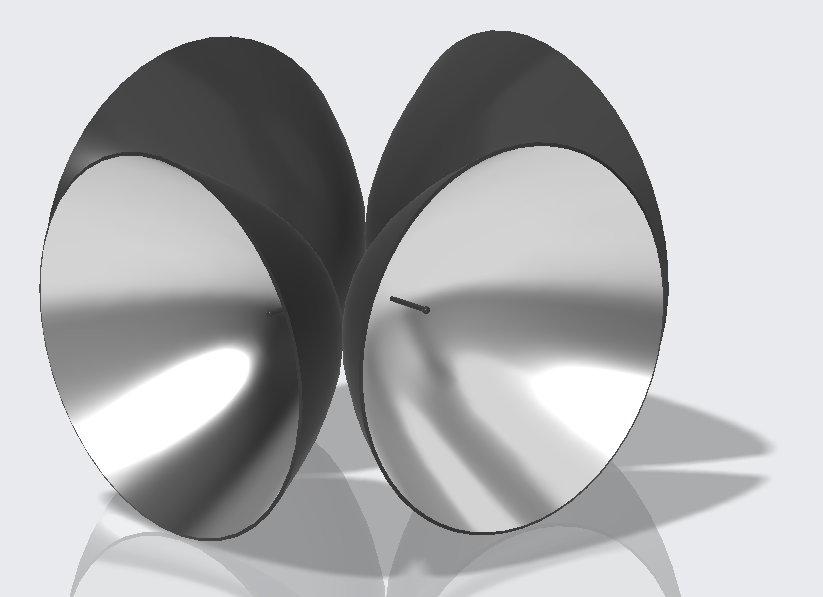
\includegraphics[width=0.65\textwidth]{figs/img/paraboloidalReflector}
    %    \caption{Quad-Parabolic Reflector Model}
    %    \label{fig:parabolodialReflector}
    %\end{figure}
\end{frame}

%----------------------------------

\subsection{Block Diagrams}
\begin{frame}{Block Diagrams}
    \begin{itemize}
        \item Two main components of system
            \begin{itemize}
                \item Mobile Cart
                \item Remote Target
            \end{itemize}
        \item System Block Diagram shown in Figure \autoref{fig:sysBlockDiag}
    \end{itemize}
    \begin{figure}[b]
        \centering
        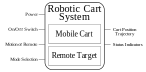
\includegraphics[width=0.8\textwidth]{figs/system_block_diagram_2}
        \caption{Block Diagram of the Robotic Cart System}
        \label{fig:sysBlockDiag}
    \end{figure}
\end{frame}

%----------------------------------

\begin{frame}{Block Diagrams}
    \begin{itemize}
        \item Mobile Cart Subsystem Block Diagram shown in Figure \autoref{fig:sysMobileBlockDiag}
    \end{itemize}
    \begin{figure}[b]
        \centering
        \includegraphics[width=0.9\textwidth]{figs/mobile_cart_block_diagram}
        \caption{Mobile Cart Block Diagram of the Robotic Cart System}
        \label{fig:sysMobileBlockDiag}
    \end{figure}
\end{frame}

%----------------------------------

\begin{frame}{Block Diagrams}
    \begin{itemize}
        \item Remote Target Subsystem Block Diagram shown in Figure \autoref{fig:sysRemoteBlockDiag}
    \end{itemize}
    \begin{figure}[b]
        \centering
        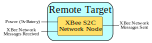
\includegraphics[width=\textwidth]{figs/remote_target_block_diagram}
        \caption{Mobile Cart Block Diagram of the Robotic Cart System}
        \label{fig:sysRemoteBlockDiag}
    \end{figure}
\end{frame}

%----------------------------------

\subsection{System Requirements}
\begin{frame}{System Requirements}
  \begin{block}{Specifications}
    \begin{itemize}
      \item Cart should be able to follow the remote while maintaining a distance of 1 to 1.5 meters.
      \item Cart should be able to travel at 1 m/s
      \item Cart should not require line-of-sight to follow remote
     \end{itemize}
  \end{block}
\end{frame}

%----------------------------------

\section{Parts List}

\begin{frame}{Parts List}

  \begin{table}[h!]
      \centering
      \begin{tabular}{c|c|c}
          \toprule
          \textbf{Quantity} & \textbf{Parts} & \textbf{Price}\\
          \toprule
          4 & Pololu 37D Metal Gaermotor 4751 & \$ 39.95\\
          12 & XBee S2C Module & \$ 23.10\\
          10 & XBee Adapter Board & \$ 4.99\\
          2 & Twotrees 4 Lead Nema 17 Stepper Motor & \$ 9.99\\
          1 & 4-Pin JST SH Connector - 20 Pack & \$ 7.99\\
          1 & 6-Pin JST SH Connector - 10 Pack & \$ 9.99\\
          1 & Aluminum Foil Tape - 2 in x 5 yd & \$ 6.05\\
          \bottomrule
          \multicolumn{2}{r|}{\textbf{Total}} & \$ 562.34\\
          \bottomrule
      \end{tabular}
      \caption{Comprised parts list for the Robotic Cart project}
      \label{tab:Partslist}
  \end{table}

\end{frame}

%----------------------------------

\begin{frame}{Parts List}

  \begin{table}[h!]
      \centering
      \begin{tabular}{c|c}
          \toprule
          \textbf{Quantity} & \textbf{Parts}\\
          \toprule
          2 & Budget Bot Chassis\\
          4 & 10 uF Ceramic Capacitor\\
          4 & LM1117 Regulator\\
          2 & Battery Packs for Budget Bot\\
          8 & 9V Batteries\\
          4 & Solderable PCB Boards\\
          3 & XBee USB Adapter\\
          \bottomrule
          %\multicolumn{2}{r|}{\textbf{Total}} & \$ 562.34\\
          %\bottomrule
      \end{tabular}
      \caption{List of laboratory parts}
      \label{tab:Partslablist}
  \end{table}

\end{frame}

%----------------------------------

\section{Timeline and Milestones}

\begin{frame}{Fall Semester}

	  \begin{figure}
      \centering
      \begin{ganttchart}[
        hgrid,
        vgrid,
        x unit=.27cm,
        y unit title=.5cm,
        y unit chart=.27cm,
        title label font=\scriptsize,
        milestone label font=\tiny,
        milestone progress label font = \tiny,
        milestone progress label anchor = east,
        bar label font=\tiny,
        group label font=\footnotesize,
        bar/.append style={fill=green},
        bar incomplete/.append style={fill=red},
        group progress label font = \tiny,
        progress label text={$\displaystyle####1\%$},
        group progress label anchor = east,
        bar progress label font = \tiny,
        bar progress label anchor = east,
        ]{1}{17}

        \gantttitle{2020}{17}\\
        \gantttitle{Sep}{4}
        \gantttitle{Oct}{4}
        \gantttitle{Nov}{4}
        \gantttitle{Dec}{4}
        \gantttitle{}{1}\\
    
        \ganttgroup[progress = 100]{Research}{3}{12} \\
        \ganttbar[progress = 100]{Research Multipath}{3}{12}\\
        \ganttbar[progress = 100]{Research Reflector}{3}{12}\\

        \ganttgroup[progress = 80]{Simulation}{8}{10}\\
        \ganttbar[progress = 80]{CoppeliaSim simulation}{8}{10}\\
        \ganttmilestone[progress = 0]{Simulation Complete}{10}\\

        \ganttgroup[progress = 55]{Project Proposal}{11}{12}\\
        \ganttbar[progress = 60]{Proposal Document}{11}{11}\\
        \ganttbar[progress = 50]{Proposal Presentation}{12}{12}\\

        \ganttgroup[progress = 12.5]{XBee Setup}{13}{14}\\
        \ganttbar[progress = 0]{Voltage Regulator Circuit}{13}{13}\\
        \ganttbar[progress = 0]{Configuration with X-CTU}{14}{14}\\
        \ganttbar[progress = 0]{Sensing RSSI}{14}{14}\\
        \ganttbar[progress = 50]{UART Communication}{14}{14}\\
      \end{ganttchart}
    \caption{Gantt chart for Fall 2020}
    \label{fig:gantt1}
  \end{figure}
	
\end{frame}

%----------------------------------

\begin{frame}{Spring Semester}
\begin{figure}
  \centering
  \begin{ganttchart}[
    hgrid,
    vgrid,
    x unit=.25cm,
    y unit title=.45cm,
    y unit chart=.25cm,
    title label font=\scriptsize,
    milestone label font=\tiny,
    milestone progress label font = \tiny,
    milestone progress label anchor = east,
    bar label font=\tiny,
    group label font=\footnotesize,
    bar/.append style={fill=green},
    bar incomplete/.append style={fill=red},
    group progress label font = \tiny,
    progress label text={$\displaystyle####1\%$},
    group progress label anchor = east,
    bar progress label font = \tiny,
    bar progress label anchor = east,
    ]{1}{20}
    \gantttitle{2020}{20}\\
    \gantttitle{Jan}{3}
    \gantttitle{Feb}{4}
    \gantttitle{Mar}{4}
    \gantttitle{Apr}{4}
    \gantttitle{May}{4}
    \gantttitle{}{1}\\

    \ganttgroup[progress = 0]{Assembly}{3}{4}\\
    \ganttbar[progress = 0]{Replace Motors}{3}{3}\\
    \ganttbar[progress = 0]{Design and Construct Reflector}{3}{4}\\
    \ganttbar[progress = 0]{Mount Reflector}{4}{4}\\
    \ganttmilestone[progress = 0]{Assembly Complete}{4}\\

    \ganttgroup[progress = 0]{Software}{5}{6}\\
    \ganttbar[progress = 0]{XBee Library}{5}{5}\\
    \ganttbar[progress = 0]{Control Algorithm}{6}{6}\\

    \ganttgroup[progress = 0]{Angle Estimation}{7}{8}\\
    \ganttbar[progress = 0]{Rotate XBee on Stepper Motor}{7}{7}\\
    \ganttbar[progress = 0]{Determine Angle}{8}{8}\\

    \ganttgroup[progress = 0]{Distance Estimation}{9}{10}\\
    \ganttbar[progress = 0]{Calibrate Distance Calculation}{9}{10}\\

    \ganttgroup[progress = 0]{Subsystem Integration}{11}{15}\\
    \ganttbar[progress = 0]{Angle Estimation Testing}{11}{11}\\
    \ganttbar[progress = 0]{Distance Estimation Testing}{12}{13}\\
    \ganttbar[progress = 0]{System Testing}{14}{15}\\
    \ganttmilestone[progress = 0]{Integration Complete}{15}\\

    \ganttgroup[progress = 0]{Project Completion}{16}{17}\\
    \ganttbar[progress = 0]{Final Report}{16}{16}\\
    \ganttbar[progress = 0]{Final Presentation}{17}{17}\\
    \ganttbar[progress = 0]{Presentation to IAB}{17}{17}\\
    \ganttbar[progress = 0]{Project Demo}{17}{17}\\

    \ganttmilestone[progress = 0]{Project Complete}{17}
  \end{ganttchart}
  \caption{Gantt Chart for Spring 2020}
  \label{fig:gantt2}
\end{figure}
\end{frame}

%----------------------------------

\section{References}

\begin{frame}{References}
	\bibliographystyle{IEEEtran}
	\begin{itemize}
		\item N. Rawashdeh, R. Haddad, O. Jadallah, and A. To’ma, “A person-following
robotic cart controlled via a smartphone application: design and evaluation,”
09 2017, pp. 1–5.
		\item M. M. Islam, A. Lam, H. Fukuda, Y. Kobayashi, and Y. Kuno, “An intelligent
shopping support robot: understanding shopping behavior from 2d skeleton data using gru network,” ROBOMECH Journal, vol. 6, no. 1, 2019.
		\item J. Sales, J. Marti, R. Marin Prades, E. Cervera, and P. Sanz, “Comparob: The
shopping cart assistance robot,” International Journal of Distributed Sensor Networks, vol. 2016, pp. 1–15, 02 2016.
		\item M. S. Miah, J. Knoll, and K. Hevrdejs, “Intelligent range-only mapping and navigation for mobile robots,” IEEE Transactions on Industrial Informatics, vol. 14, no. 3, pp. 1164–1174, 2018.
		\item D. Li and S. Lane, “A novel and versatile parabolic reflector that significantly
improves wi-fi reception at different distances and angles,” 2013.
	
	\end{itemize}


\end{frame}

%----------------------------------

\begin{frame}{References}

	\bibliographystyle{IEEEtran}
	\begin{itemize}
		\item T. Xie, H. Jiang, X. Zhao, and C. Zhang, “A wi-fi-based wireless indoor position sensing system with multipath interference mitigation,” Sep 2019. [Online].
Available: https://www.ncbi.nlm.nih.gov/pmc/articles/PMC6767237/
		\item A. M. Ladd, K. E. Bekris, A. Rudys, L. E. Kavraki, and D. S. Wallach, “Robotics-
based location sensing using wireless ethernet,” Wireless Networks, vol. 11, no. 1-2, p. 189–204, 2005.
		\item M. Lindhe, K. Johansson, and A. Bicchi, “An experimental study of exploiting multipath fading for robot communications,” Robotics: Science and Systems III, 2007.
		\item M. Lindhe and K. Johansson, “Using robot mobility to exploit multipath fading,”Wireless Communications, IEEE, vol. 16, pp. 30 – 37, 03 2009.
	\end{itemize}

\end{frame}

%----------------------------------

% \begin{frame}{Introduction}{}
% \begin{figure}
%   \centering
%   \includegraphics[scale=0.31]{figs/ipe/highLevel_wht_grn}
%   \caption{General high-level system architecture}
%   \label{fig:ProblemStatementImage}
% \end{figure}
% \end{frame}

% \begin{frame}{Introduction}{}
%         \begin{itemize}
%         \item This project will:
%             \begin{itemize}
%                 \item use a pair of 2-DOF (2-degrees-of-freedom) mechatronics platforms
%                 \item implement control algorithms on embedded system
%                 \item use mobile device for user control
%                 \item encourage research
%                 \item serve as an educational tool
%             \end{itemize}
%         \end{itemize}
% \end{frame}

% %----------------------------------

% \section{Background Study}

% \subsection{Control Techniques}

% \begin{frame}{Background Study}{Control Techniques}
%     Various control techniques have been proposed for 2-DOF helicopters such as:
%     \begin{itemize}
%         \item Sliding mode control \cite{Ahmed2010-Sliding} %cite 2-Sliding Mode Based Robust Control for 2-DOF Helicopter here
%         \item Fuzzy Logic control 
%         \cite{Chang2017-Fuzzy}
%         \cite{Kayacan2016-Fuzzy}
%         \cite{Mendez-Monroy2012-Fuzzy} 
%         %cite Fuzzy control with estimated variable sampling period for non-linear networked control systems: 2-DOF helicopter as case study here
%         \item Data-driven Adaptive Optimal Output-feedback control \cite{Gao2016-DataDriven} %cite Data-driven Adaptive Optimal Output-feedback Control of a 2-DOF Helicopter here
%         \item Decentralized discrete-time neural control \cite{Hernandez-Gonzalez2012-Decentralized} %cite Decentralized discrete-time neural control for a Quanser 2-DOF helicopter here
%     \end{itemize}
%     These control techniques employ advanced mathematics that are difficult to implement on embedded systems.
% \end{frame}

% %----------------------------------

% \subsection{Modeling a 2-DOF Helicopter}

% \begin{frame}{Background Study}{Modeling a 2-DOF Helicopter}
%     \begin{columns}
%     \column{0.5\textwidth}
%     \begin{figure}
%         \centering
%         \includegraphics[width=\textwidth]{figs/img/helicopterModel}
%         \caption{Model of a 2-DOF helicopter}
%         \label{fig:helicopterModel}
%     \end{figure}
%     \column{0.5\textwidth}
%     \begin{figure}
%       \centering 
%       \includegraphics[width=\textwidth]{figs/img/QuanserAero}
%       \caption{Quanser Aero}
%       \label{fig:QuanserAero}
%     \end{figure}    
%     \end{columns}
% \end{frame}

% \begin{frame}{Background Study}{Modeling a 2-DOF Helicopter}
%     \begin{itemize}
%         \item Characterized by fixed base
%         \begin{itemize}
%             \item Can change 2 of 3 possible orientations...
%             \begin{itemize}
%                 \item Pitch ($\theta$)
%                 \item Yaw ($\psi$)
%                 \item \emph{Not Roll}
%             \end{itemize}
%             \item and cannot change position
%             \begin{itemize}
%                 \item x direction
%                 \item y direction
%                 \item z direction
%             \end{itemize}
%         \end{itemize} 
%     \end{itemize}
% \end{frame}

% % \begin{frame}{Background Study}{Quanser Aero} 

% % \end{frame}

% \begin{frame}{Background Study}{Modeling a 2-DOF Helicopter}
%     \begin{itemize}
%         \item Motors are attached to the propellers to create thrust due to air resistance
%             \begin{itemize}
%                 \item Main - changes pitch angle
%                 \item Tail - changes yaw angle
%             \end{itemize} 
%         \item Torque due to rotation also creates a force on opposite axes 
%     \end{itemize}
% \end{frame}

% \begin{frame}{Background Study}{Modeling a 2-DOF Helicopter}
% Due to the efficiency of the Quanser Aero, we can create a linearized system model:
% \begin{align}
%   %\dot{\bf x}(t) = {\bf A}{\bf x}(t) +{\bf B}{\bf u}(t),~\mathrm{where}
%     \dot{\bf x}(t) = {\bf A}{\bf x}(t) +{\bf B}{\bf u}(t),~\mathrm{such}~\mathrm{that}
% \label{eq:stateModel}
% \end{align}  
% %
% \begin{align*}
% \begin{bmatrix}
%     \dot\theta\\
%     \dot\psi\\
%     \ddot{\theta}\\
%     \ddot{\psi}
% \end{bmatrix}&=
% %\label{eq:matrixA}
% \begin{bmatrix}
%     0 & 0 & 1 & 0 \\
%     0 & 0 & 0 & 1 \\
%     0 & -K_{sp}/J_p & -D_p/J_p & 0 \\
%     0 & 0 & 1 & -D_y/J_y 
% \end{bmatrix} 
% %\label{eq:stateMatrix} 
% \begin{bmatrix}
%     \theta\\
%     \psi\\
%     \dot{\theta}\\
%     \dot{\psi}
% \end{bmatrix}
% \\&+
% %\label{eq:matrixB}
% \begin{bmatrix}
%     0 & 0 \\
%     0 & 0 \\
%     K_{pp}/J_p & K_{py}/J_p \\
%     K_{yp}/J_y & K_{yy}/J_y 
% \end{bmatrix}
% %\label{eq:inputMatrix}
% \begin{bmatrix}
%     V_p \\
%     V_y 
% \end{bmatrix}
% %{\bf A} =  
% %\begin{bmatrix}
% %0 & 0 & 1 & 0\\
% %0 & 0 & 0 & 1\\
% %-\frac{K_{\text{sp}}}{J_p} & 0 & -\frac{D_p}{J_p} &  0\\
% %0 & 0 & 0 & -\frac{D_y}{J_y}    
% %\end{bmatrix}
% %~\text{and}~
% %  {\bf B} =
% %\begin{bmatrix}
% %0 & 0\\
% %0 & 0\\
% %\frac{K_{\text{pp}}}{J_p} & \frac{K_{\text{py}}}{J_p}\\
% %\frac{K_{\text{yp}}}{J_y} & \frac{K_{\text{yy}}}{J_y}                           
% %\end{bmatrix}
% \end{align*}
% \end{frame}

% \begin{frame}{Background Study}{Modeling a 2-DOF Helicopter}
% \begin{itemize}
%     \item $K_{sp}$ - being the stiffness of the axes
%     \item $K_{pp}$ - pitch motor thrust constant
%     \item $K_{py}$ - thrust constant acting on the pitch angle from the yaw motor
%     \item $K_{yp}$ - thrust constant acting on the yaw angle from the pitch motor
%     \item $K_{yy}$ - yaw motor thrust constant
%     \item $J_p$ - moment of inertia about pitch axis
%     \item $J_y$ - moment of inertia about yaw axis
%     \item $D_p$ - viscous damping of the pitch axis
%     \item $D_y$ - viscous damping of the yaw axis
% \end{itemize}
% \end{frame}

% %----------------------------------
% \subsection{Control Algorithm and Architecture}
% \begin{frame}{Background Study}{Control Algorithm Overview - Optimal Control}
% \begin{enumerate}
%     \item Employ state-space representation of 2-DOF helicopter:
%     \begin{align*}
%         \dot{\mathbf{x}} = \mathbf{A}\mathbf{x} + \mathbf{B}\mathbf{u}
%     \end{align*}
%     \item Use state feedback law
%     \begin{center}
%         $\mathbf{u} = -\mathbf{K}\mathbf{x}$
%     \end{center}
%     to minimize the quadratic cost function:
%     \begin{align*}
%         J(\mathbf{u}) = \int_0^\infty (\mathbf{x}^T\mathbf{Q}\mathbf{x} + \mathbf{u}^T\mathbf{R}\mathbf{u} + 2\mathbf{x}^T\mathbf{N}\mathbf{u})\mathrm{dt}
%     \end{align*}
%     \item Find the solution $\mathbf{S}$ to the Riccati equation
%     \begin{align*}
%         \mathbf{A}^T\mathbf{S}+\mathbf{SA}-(\mathbf{SB}+\mathbf{N})\mathbf{R}^{-1}(\mathbf{B}^T\mathbf{S}+\mathbf{N}^T)+\mathbf{Q}=0
%     \end{align*}    
%     \item Calculate gain, $\mathbf{K}$
%     \begin{center}
%         $\mathbf{K}=\mathbf{R}^{-1}(\mathbf{B}^T\mathbf{S}+\mathbf{N}^T)$
%     \end{center}
% \end{enumerate}
% \end{frame}
% %----------------------------------
% \begin{frame}{Background Study}{Control Algorithm Overview - Optimal Noise Resistant Control}
% \begin{itemize}
%     \item Utilizes gain calculated in LQR
%     \item Added Kalman filter to reduce external disturbances to the system
% \end{itemize} 
% \begin{figure}
%     \centering
%     \includegraphics[width=.8\textwidth,keepaspectratio=true]{figs/img/LQG_SimulinkResize.png}
%     \caption{Noise resistant 2-DOF helicopter model}
%     \label{fig:LQGModel}
% \end{figure}
% \end{frame}
% %----------------------------------
% \begin{frame}{Background Study}{Control Algorithm Overview - Machine Learning}
%     \begin{columns}
%     \column{0.5\textwidth}
%     \begin{figure}
%         \centering
%         \includegraphics[width=\textwidth]{figs/ipe/ADP_Neural_Network}
%         \caption{Neural network}
%         \label{fig:ADP_Neural_Networkl}
%     \end{figure}
%     \column{0.5\textwidth}
%     \begin{figure}
%       \centering 
%       \includegraphics[width=\textwidth]{figs/ipe/ADP_Samples}
%       \caption{Neural network sampling}
%       \label{fig:ADP_Samples}
%     \end{figure}    
%     \end{columns}
% \end{frame}
% %----------------------------------
% \begin{frame}{Background Study}{Control Architecture Overview -  P Type Controller}
% \begin{figure}
%     \centering
%     \includegraphics[width=.8\textwidth,keepaspectratio=true]{figs/ipe/P_Control}
%     \caption{Optimal P type controller [servo]}
%     \label{fig:P_Control}
% \end{figure}
% \end{frame}
% %----------------------------------
% \begin{frame}{Background Study}{Control Architecture Overview - PI Type Controller}
% \begin{figure}
%     \centering
%     \includegraphics[width=.8\textwidth,keepaspectratio=true]{figs/ipe/PI_Control}
%     \caption{Optimal PI type controller [servo]}
%     \label{fig:PI_Control}
% \end{figure}
% \end{frame}
% %----------------------------------

% \subsection{Prior Work}

% \begin{frame}{Background Study}{Prior Work}
%   \begin{itemize}
%       \item extensive modeling \& simulations
%       \item implementation of two motion control algorithms (LQR \& ADP)
%       \item one helicopter
%       %\item deployed on mobile device
%   \end{itemize}
% \end{frame}

% %----------------------------------

% % \subsection{Challenges}

% % \begin{frame}{Background Study}{Challenges}
  
% % \end{frame}

% %----------------------------------

% \section{Subsystem Level Functional Requirements}

% % put a slide with three dimensional system architecture drawing using ipe
% % another slide with explanation

% % put a slide with system block diagram

% \subsection{Block Diagram}

% \begin{frame}{Subsystem Level Functional Requirements}{Block Diagram}

% \begin{figure}
%   \centering
%   \includegraphics[scale=0.31]{figs/ipe/TCPModel}
%   \caption{Communication model}
%   \label{fig:TCPModel}
% \end{figure}

% \end{frame}

% \begin{frame}{Subsystem Level Functional Requirements}{Block Diagram} 

% \begin{figure}
%   \centering 
%   \includegraphics[scale=0.31]{figs/ipe/lowLevel}
%   \caption{Low level smart control diagram}
%   \label{fig:ProposalImage}
% \end{figure}

% \end{frame}

% %----------------------------------

% \section{Simulation}

% \subsection{Optimal Control Simulation}

% % P Controller
% \begin{frame}{Simulation}{Optimal Control Simulation (P Type Controller)}
%     \begin{figure}
%       \centering
%       \subfigure[][]{
%         \label{fig:LQR_Pos_Con}
%         \includegraphics[scale=0.38]{figs/MATLAB/LQR/P_Simulation/LQR_Pos_Con}
%       }
%       \subfigure[][]{
%         \label{fig:LQR_Volt_Con}
%         \includegraphics[scale=0.38]{figs/MATLAB/LQR/P_Simulation/LQR_Volt_Con}    
%       }  
%       \caption{Optimal control (P type controller) simulation \subref{fig:LQR_Pos_Con}~position and~\subref{fig:LQR_Volt_Con}~voltage w/ step input}
%       \label{fig:LQR_Sim_Con}
%     \end{figure}
% \end{frame}

% \begin{frame}{Simulation}{Optimal Control Simulation (P Type Controller)}
%     \begin{figure}
%       \centering 
%       \includegraphics[scale=0.5]{figs/MATLAB/LQR/P_Simulation/LQR_Error_Con}
%       \caption{Optimal control (P type controller) simulation w/ constant signal}
%       \label{fig:LQR_Error_Con}
%     \end{figure}
% \end{frame}

% % PI LQR vs LQG
% \subsection{Noise Resistant and Optimal Control Simulation}
% \begin{frame}{Simulation}{Noise Resistant and Optimal Control (PI type Controller) Simulation}
%     \begin{figure}
%       \centering
%       \subfigure[][]{
%         \label{fig:Pitch}
%         \includegraphics[scale=0.38]{figs/matlab/LQG_PIvLQR_PI_Sim/Pitch}
%       }
%       \subfigure[][]{
%         \label{fig:Yaw}
%         \includegraphics[scale=0.38]{figs/matlab/LQG_PIvLQR_PI_Sim/Yaw}    
%       }  
%       \caption{Noise resistant control vs optimal control (PI type controller) simulation \subref{fig:Pitch}~pitch~position and~\subref{fig:Yaw}~yaw~position w/ step input}
%       \label{fig:LQR_LQG_Sim_pos}
%     \end{figure}
% \end{frame}

% \begin{frame}{Simulation}{Noise Resistant and Optimal Control (PI Type Controller) Simulation}
%     \begin{figure}
%       \centering
%       \subfigure[][]{
%         \label{fig:Pitch_Volt}
%         \includegraphics[scale=0.38]{figs/matlab/LQG_PIvLQR_PI_Sim/Pitch_Volt}
%       }
%       \subfigure[][]{
%         \label{fig:Yaw_Volt}
%         \includegraphics[scale=0.38]{figs/matlab/LQG_PIvLQR_PI_Sim/Yaw_Volt}    
%       }  
%       \caption{Noise resistant control vs optimal control (PI type controller) simulation \subref{fig:Pitch_Volt}~pitch~voltage and~\subref{fig:Yaw_Volt}~yaw~voltage w/ step input}
%       \label{fig:LQR_PI_Sim_volt}
%     \end{figure}
% \end{frame}

% %% PI Controller
% %\begin{frame}{Simulation}{Optimal Control Simulation (PI Controller)}
% %    \begin{figure}
% %      \centering
% %      \subfigure[][]{
% %        \label{fig:Pitch_LQR_Sim}
% %        \includegraphics[scale=0.38]{figs/MATLAB/LQR/PI_Sim/Pitch_LQR_Sim}
% %      }
% %      \subfigure[][]{
% %        \label{fig:Yaw_LQR_Sim}
% %        \includegraphics[scale=0.38]{figs/MATLAB/LQR/PI_Sim/Yaw_LQR_Sim}    
% %      }  
% %      \caption{Optimal Control (PI Controller) Simulation \subref{fig:Pitch_LQR_Sim}~Pitch~Position and~\subref{fig:Yaw_LQR_Sim}~Yaw~Position w/ Step Input}
% %      \label{fig:LQR_PI_Sim_pos}
% %    \end{figure}
% %\end{frame}
% %
% %\begin{frame}{Simulation}{Optimal Control (PI Controller) Simulation}
% %    \begin{figure}
% %      \centering
% %      \subfigure[][]{
% %        \label{fig:Pitch_Volt_LQR_Sim}
% %        \includegraphics[scale=0.38]{figs/MATLAB/LQR/PI_Sim/Pitch_Volt_LQR_Sim}
% %      }
% %      \subfigure[][]{
% %        \label{fig:Yaw_Volt_LQR_Sim}
% %        \includegraphics[scale=0.38]{figs/MATLAB/LQR/PI_Sim/Yaw_Volt_LQR_Sim}    
% %      }  
% %      \caption{Optimal Control (PI Controller) Simulation \subref{fig:Pitch_Volt_LQR_Sim}~Pitch~Voltage and~\subref{fig:Yaw_Volt_LQR_Sim}~Yaw~Voltage w/ Step Input}
% %      \label{fig:LQR_PI_Sim_volt}
% %    \end{figure}
% %\end{frame}
% %
% %% LQG
% %\subsection{Optimal Noise Resistant Control Simulation}
% %\begin{frame}{Simulation}{Optimal Noise Resistant Control (PI Controller) Simulation}
% %    \begin{figure}
% %      \centering
% %      \subfigure[][]{
% %        \label{fig:Pitch_LQG_Sim}
% %        \includegraphics[scale=0.38]{figs/MATLAB/LQG/LQG_Sim/Pitch_LQG_Sim}
% %      }
% %      \subfigure[][]{
% %        \label{fig:Yaw_LQG_Sim}
% %        \includegraphics[scale=0.38]{figs/MATLAB/LQG/LQG_Sim/Yaw_LQG_Sim}    
% %      }  
% %      \caption{Optimal Noise Resistant Control (PI Controller) \subref{fig:Pitch_LQG_Sim}~Pitch~Position and~\subref{fig:Yaw_LQG_Sim}~Yaw~Position w/ Step Input}
% %      \label{fig:LQG_PI_Sim_pos}
% %    \end{figure}
% %\end{frame}
% %
% %\begin{frame}{Simulation}{Optimal Noise Resistant Control (PI Controller) Simulation}
% %    \begin{figure}
% %      \centering
% %      \subfigure[][]{
% %        \label{fig:Pitch_Volt_LQG_Sim}
% %        \includegraphics[scale=0.38]{figs/MATLAB/LQG/LQG_Sim/Pitch_Volt_LQG_Sim}
% %      }
% %      \subfigure[][]{
% %        \label{fig:Yaw_Volt_LQG_Sim}
% %        \includegraphics[scale=0.38]{figs/MATLAB/LQG/LQG_Sim/Yaw_Volt_LQG_Sim}    
% %      }  
% %      \caption{Optimal Noise Resistant Control Simulation (PI Controller) \subref{fig:Pitch_Volt_LQG_Sim}~Pitch~Voltage and~\subref{fig:Yaw_Volt_LQG_Sim}~Yaw~Voltage w/ Step Input}
% %      \label{fig:LQG_PI_Sim_volt}
% %    \end{figure}
% %\end{frame}

% %----------------------------------

% \section{Implementation}

% \subsection{USB}
% %LQR
% \begin{frame}{Implementation}{Optimal Control P and PI Type Controller USB}
%     \begin{figure}
%       \centering
%       \subfigure[][]{
%         \label{fig:Pitch_LQR_RMSE}
%         \includegraphics[scale=0.38]{figs/matlab/LQR_PIvLQR_P_USB/step/Pitch_LQR_RMSE}
%       }
%       \subfigure[][]{
%         \label{fig:Yaw_LQR_RMSE}
%         \includegraphics[scale=0.38]{figs/matlab/LQR_PIvLQR_P_USB/step/Yaw_LQR_RMSE}    
%       }  
%       \caption{USB implementation comparison between optimal control (P~type~controller) and optimal control (PI~type~controller) for \subref{fig:Pitch_LQR_RMSE}~pitch and \subref{fig:Yaw_LQR_RMSE}~yaw configurations w/ step input}
%       \label{fig:PvPI_USB}
%     \end{figure}
% \end{frame}
% %
% \begin{frame}{Implementation}{Optimal Control P and PI Type Controller USB}
%     \begin{figure}
%       \centering
%       \subfigure[][]{
%         \label{fig:PitchVoltage_LQR_RMSE}
%         \includegraphics[scale=0.38]{figs/matlab/LQR_PIvLQR_P_USB/step/PitchVoltage_LQR_RMSE}
%       }
%       \subfigure[][]{
%         \label{fig:YawVoltage_LQR_RMSE}
%         \includegraphics[scale=0.38]{figs/matlab/LQR_PIvLQR_P_USB/step/YawVoltage_LQR_RMSE}    
%       }  
%       \caption{USB implementation comparison between optimal control (P~type~controller) and optimal control (PI~type~controller) for \subref{fig:PitchVoltage_LQR_RMSE}~pitch and \subref{fig:YawVoltage_LQR_RMSE}~yaw voltages w/ step input}
%       \label{fig:PvPIVoltage_USB}
%     \end{figure}
% \end{frame}
% %
% \begin{frame}{Implementation}{Optimal Control P and PI Type Controller USB}
% \begin{table}
%     \centering
%     \begin{tabular}{l|l|l}
%         \toprule
%         \textbf{} & \textbf{Pitch Step} & \textbf{Yaw Step}\\
%         \toprule
%         LQR P & 3.5025 & 5.8502\\
%         LQR PI & 1.2349 & 5.5058\\
%         Improvement & 64.7437\% & 0.5408\% \\
%         \toprule
%         \textbf{} & \textbf{Pitch Square} & \textbf{Yaw Square}\\
%         \toprule
%         LQR P & 6.2819 & 20.4623\\
%         LQR PI & 6.9206 & 21.0709\\
%         Improvement & -10.1675\% & -2.9740\% \\
%         \toprule
%         \textbf{} & \textbf{Pitch Sine} & \textbf{Yaw Sine}\\
%         \toprule
%         LQR P & 4.2469 & 2.8644\\
%         LQR PI & 1.3383 & 1.7852\\
%         Improvement & 68.4872\% & 63.2998\% \\
%     \end{tabular}
%     \caption{Root mean squared error}
%     \label{tab:RMSE}
% \end{table}
% \end{frame}
% %\begin{frame}{Implementation}{Optimal Control P and PI Controller USB}
% %\begin{table}
% %    \centering
% %    \begin{tabular}{l|l|l|l|l|l|l}
% %        \toprule
% %        \textbf{0} & \textbf{Pitch Step} & \textbf{Yaw Step} & \textbf{Pitch Square} & \textbf{Yaw Square} & \textbf{Pitch Sine} & \textbf{Yaw Sine}\\
% %        \toprule
% %        LQR P & 3.5025 & 5.8502 & 6.2819 & 20.4623 & 4.2469 & 2.8644\\
% %        LQR PI & 1.2349 & 5.5058 & 6.9206 & 21.0709 & 1.3383 & 1.7852
% %        \bottomrule
% %    \end{tabular}
% %    \caption{Root Mean Squared Error}
% %    \label{tab:RMSE}
% %\end{table}
% %\end{frame}
% %Machine vs LQR
% \begin{frame}{Implementation}{Machine Learning and Optimal Control (P Type Controller) USB}
%     \begin{figure}
%       \centering
%       \subfigure[][]{
%         \label{fig:Pitch_LQRvADP_USB}
%         \includegraphics[scale=0.38]{figs/matlab/ADPvLQR_P_USB/Pitch_ADP_LQR}
%       }
%       \subfigure[][]{
%         \label{fig:Yaw_LQRvADP_USB}
%         \includegraphics[scale=0.38]{figs/matlab/ADPvLQR_P_USB/Yaw_ADP_LQR}    
%       }  
%       \caption{USB implementation comparison between machine learning and optimal control (P type controller) for \subref{fig:Pitch_LQRvADP_USB}~pitch and \subref{fig:Yaw_LQRvADP_USB}~yaw orientations w/ step input}
%       \label{fig:LQRvADP_USB}
%     \end{figure}
% \end{frame}
% \begin{frame}{Implementation}{Machine Learning and Optimal Control (P Type Controller) USB}
% \begin{table}
%     \centering
%     \begin{tabular}{l|l|l}
%         \toprule
%         \textbf{} & \textbf{Pitch Step} & \textbf{Yaw Step}\\
%         \toprule
%         ADP P & 1.3067 & 6.1991\\
%         LQR P & 3.5025 & 5.8502\\
%         Improvement & 62.6923\% & -5.9638\% \\
%         \toprule
%         \textbf{} & \textbf{Pitch Square} & \textbf{Yaw Square}\\
%         \toprule
%         ADP P & 6.5790 & 21.1923\\
%         LQR P & 6.2819 & 20.4623\\
%         Improvement & -4.7294\% & -0.3567\% \\
%         \toprule
%         \textbf{} & \textbf{Pitch Sine} & \textbf{Yaw Sine}\\
%         \toprule
%         ADP P & 2.1877 & 3.6307\\
%         LQR P & 4.2469 & 2.8644\\
%         Improvement & 48.4871\% & -26.7525\% \\
%     \end{tabular}
%     \caption{Root mean squared error}
%     \label{tab:RMSE2}
% \end{table}
% \end{frame}
% \subsection{Android}
% %LQR
% \begin{frame}{Implementation}{Optimal Control (P Type Controller) via Android}
%     \begin{figure}
%       \centering
%       \subfigure[][]{
%         \label{fig:LQR_Pitchpos}
%         \includegraphics[scale=0.38]{figs/matlab/LQR/P_Android/LQR_Pitchpos}
%       }
%       \subfigure[][]{
%         \label{fig:LQR_Yawpos}
%         \includegraphics[scale=0.38]{figs/matlab/LQR/P_Android/LQR_Yawpos}    
%       }  
%       \caption{Optimal control (P type controller) \subref{fig:LQR_Pitchpos}~pitch~position and~\subref{fig:LQR_Yawpos}~yaw~position w/ input from mobile phone}
%       \label{fig:LQR_pos}
%     \end{figure}
% \end{frame}
% %
% \begin{frame}{Implementation}{Optimal Control (P Type Controller) via Android}
%     \begin{figure}
%       \centering
%       \subfigure[][]{
%         \label{fig:LQR_PitchVolt}
%         \includegraphics[scale=0.38]{figs/matlab/LQR/P_Android/LQR_PitchVolt}
%       }
%       \subfigure[][]{
%         \label{fig:LQR_YawVolt}
%         \includegraphics[scale=0.38]{figs/matlab/LQR/P_Android/LQR_YawVolt}    
%       }  
%       \caption{Optimal control (P type controller) \subref{fig:LQR_PitchVolt}~pitch~voltage and~\subref{fig:LQR_YawVolt}~yaw~voltage w/ input from mobile phone}
%       \label{fig:LQR_Volt}
%     \end{figure}
% \end{frame}
% %ADP
% \begin{frame}{Implementation}{Machine Learning via Android}
%     \begin{figure}
%       \centering
%       \subfigure[][]{
%         \label{fig:ADP_Pitch_Wireless}
%         \includegraphics[scale=0.38]{figs/matlab/ADP/Android/ADP_Pitch_Wireless}
%       }
%       \subfigure[][]{
%         \label{fig:ADP_Yaw_Wireless}
%         \includegraphics[scale=0.38]{figs/matlab/ADP/Android/ADP_Yaw_Wireless}    
%       }  
%       \caption{Machine learning \subref{fig:ADP_Pitch_Wireless}~pitch~position and~\subref{fig:ADP_Yaw_Wireless}~yaw~position w/ input from mobile phone}
%       \label{fig:ADP_Wireless}
%     \end{figure}
% \end{frame}
% %
% \begin{frame}{Implementation}{Machine Learning via Android}
%     \begin{figure}
%       \centering
%       \subfigure[][]{
%         \label{fig:ADP_Pitch_Volt_Wireless}
%         \includegraphics[scale=0.38]{figs/matlab/ADP/Android/ADP_Pitch_Volt_Wireless}
%       }
%       \subfigure[][]{
%         \label{fig:ADP_Yaw_Volt_Wireless}
%         \includegraphics[scale=0.38]{figs/matlab/ADP/Android/ADP_Yaw_Volt_Wireless}    
%       }  
%       \caption{Machine learning \subref{fig:ADP_Pitch_Volt_Wireless}~pitch~voltage and~\subref{fig:ADP_Yaw_Volt_Wireless}~yaw~voltage w/ input from mobile phone}
%       \label{fig:ADP_Volt_Wireless}
%     \end{figure}
% \end{frame}

% %----------------------------------
% %
% %\section{Parts List}
% %
% %\begin{frame}{Parts List}{}
% %
% %  \begin{itemize}
% %      \item Hardware
% %      \begin{itemize}
% %        \item Two Quanser Aeros
% %            \begin{itemize}
% %                \item Q-flex2 Embedded Panel
% %            \end{itemize}
% %        \item Two Single Board Computers (Raspberry Pi 3 Model B)
% %        \item Android Smart-phone or Tablet\\
% %        (Note that Apple devices could also be used, however modifications are needed)
% %      \end{itemize}
% %      \item Software
% %      \begin{itemize}
% %          \item MATLAB \& Simulink
% %          \begin{itemize}
% %            \item Raspberry Pi Support Package
% %            \item Android Support Package
% %          \end{itemize}
% %          \item Quanser Real-Time Control (QUARC)
% %          % "Quanser’s QUARC™ software adds powerful tools and capabilities to Simulink® that make the development and deployment of sophisticated real-time mechatronics and control applications easier. QUARC™ generates real-time code directly from Simulink-designed controllers and runs it in real-time on the Windows target – all without digital signal processing or without writing a single line of code."
% %      \end{itemize}
% %  \end{itemize}
% %\end{frame}

% %----------------------------------



% \section{Future Directions}

% \begin{frame}{Future Directions}{} 
%   \begin{itemize}
%     \item Discretization of System   
%     \item Digital Compass
%     \item Enhanced Smart Control
% 	\vskip .2cm
% 	\begin{figure}
% 	  \centering
% 	  \includegraphics[scale=0.28]{figs/ipe/smartAlg}
% 	  \caption{Enhanced smart control}
% 	  \label{fig:smartAlg}
% 	\end{figure}
% 	%\vskip -.4cm
%     \item Implmentation on 6-DOF Helicopter
%   \end{itemize}
% \end{frame}

% % You can reveal the parts of a slide one at a time
% % with the \pause command:
% %\begin{frame}{Second Slide Title}
% %  \begin{itemize}
% %  \item {
% %    First item.
% %    \pause % The slide will pause after showing the first item
% %  }
%   %\item {   
%   %  Second item.
%  % }
%   % You can also specify when the content should appear
%   % by using <n->:
%  % \item<3-> {
%  %   Third item.
%  % }
% %  \item<4-> {
% %    Fourth item.
%  % }
%   % or you can use the \uncover command to reveal general
%   % content (not just \items):
% %  \item<5-> {
% %    Fifth item. \uncover<6->{Extra text in the fifth item.}
% %  }
% %  \end{itemize}
% %\end{frame}

% %\section{Second Main Section}

% % \subsection{Another Subsection}

% % \begin{frame}{Blocks}
% % \begin{block}{Block Title}
% % You can also highlight sections of your %presentation in a block, with it's own %title
% % \end{block}
% % \begin{theorem}
% % There are separate environments for %theorems, examples, definitions and proofs.
% % \end{theorem}
% % \begin{example}
% % Here is an example of an example block.
% % \end{example}
% % \end{frame}

% % Placing a * after \section means it will not show in the
% % outline or table of contents.
% \section*{Summary}
% \begin{frame}{Summary} %Glenn
%   \begin{itemize}
%     \item Embedded implementation of control algorithms
%     \item Mobile interface
%     \item PI type control improves steady-state error
%     \item Machine Learning is best when system parameters are unknown or time-varient
%     %\item\todo[inline]{Add table for RMSE?}
%   \end{itemize}
  
% %   \begin{itemize}
% %   \item Outlook
% %     \begin{itemize}
% %     \item Implementation using two more motion control algorithms (LQG \& ADP)
% %     \item Development of a test plan to compare algorithms
% %     \end{itemize}
% %   \end{itemize}
% \end{frame}
% % \begin{frame}{Summary}
% %   \begin{itemize}
% %   \item
% %     The \alert{first main message} of your talk in one or two lines.
% %   \item
% %     The \alert{second main message} of your talk in one or two lines.
% %   \item
% %     Perhaps a \alert{third message}, but not more than that.
% %   \end{itemize}
  
% %   \begin{itemize}
% %   \item
% %     Outlook
% %     \begin{itemize}
% %     \item
% %       Something you haven't solved.
% %     \item
% %       Something else you haven't solved.
% %     \end{itemize}
% %   \end{itemize}
% % \end{frame}

% \section*{Acknowledgement}
%   \begin{frame}{Acknowledgement} 
%     \centering
%     Special Thanks to Andrew Fandel, Anthony Birge, and Dr. Suruz Miah for their work with Machine Learning on a 2-DOF Helicopter
%   \end{frame}

% All of the following is optional and typically not needed. 
% \appendix
% \section<presentation>*{\appendixname}
% \subsection<presentation>*{For Further Reading}

% \begin{frame}[allowframebreaks]
%   \frametitle<presentation>{For Further Reading}
%   \bibliographystyle{IEEEtran}
%   \bibliography{bib/references,bib/refsHelicopter}
  
%   \begin{thebibliography}{10}
    
%   \beamertemplatebookbibitems
%   % Start with overview books.
    
    
%   \beamertemplatearticlebibitems
 
%   % Followed by interesting articles. Keep the list short. 
    
%     \bibitem{Article1}
% M. Hernandez-Gonzalez, A.Y. Alanis, E.A. Hernandez-Vargas,
% \emph{Decentralized discrete-time neural control for a Quanser 2-DOF helicopter }.
% 2012

% \bibitem{Article2}
% F. Dos Santos Barbosa,
% \emph{4DOF quadcopter: development, modeling and control }.
% 2017

% \bibitem{Article3}
% G.G. Neto, F.S. Barbosa, B.A. Ang\'{e}lico,
% \emph{2-DOF helicopter controlling by pole-placements }.

% \bibitem{Article4}
% Weinan Gao and Zhong-Ping Jiang
% \emph{Data-driven Adaptive Optimal Output-feedback Control of a 2-DOF Helicopter }.

% \bibitem{Article5}
% P. Méndez-Monroy, H. Benítez-Pérez,
% \emph{Fuzzy Control with Estimated Variable Sampling Period for Non-Linear Networked Control Systems: 2-DOF Helicopter as Case Study }. 
% Transactions of the Institute of Measurement \& Control 34, no. 7 (October 15, 2012): 802–14. 
    
%     \bibitem{Article6}
%     Q. Ahmed and A.I.Bhatti and S.Iqbal and I.H. Kazmi
%     \emph{2-Sliding Mode Based Robust Control for 2-DOF Helicopter}.
    
% %   \bibitem{Someone2000}
% %     S.~Someone.
% %     \newblock On this and that.
% %     \newblock {\em Journal of This and That}, 2(1):50--100,
% %     2000.
%   \end{thebibliography}
% \end{frame}

\end{document}



%%% Local Variables:
%%% mode: latex
%%% TeX-master: t
%%% End:
